\documentclass[a4paper]{article}
\usepackage{lmodern}
\usepackage{amssymb,amsmath}
\usepackage{ifxetex,ifluatex}
\usepackage{fixltx2e} % provides \textsubscript
\ifnum 0\ifxetex 1\fi\ifluatex 1\fi=0 % if pdftex
  \usepackage[T1]{fontenc}
  \usepackage[utf8]{inputenc}
\else % if luatex or xelatex
  \ifxetex
    \usepackage{mathspec}
    \usepackage{xltxtra,xunicode}
  \else
    \usepackage{fontspec}
  \fi
  \defaultfontfeatures{Mapping=tex-text,Scale=MatchLowercase}
  \newcommand{\euro}{€}
\fi
% use upquote if available, for straight quotes in verbatim environments
\IfFileExists{upquote.sty}{\usepackage{upquote}}{}
% use microtype if available
\IfFileExists{microtype.sty}{%
\usepackage{microtype}
\UseMicrotypeSet[protrusion]{basicmath} % disable protrusion for tt fonts
}{}
\usepackage[margin=1in]{geometry}
\ifxetex
  \usepackage[setpagesize=false, % page size defined by xetex
              unicode=false, % unicode breaks when used with xetex
              xetex]{hyperref}
\else
  \usepackage[unicode=true]{hyperref}
\fi
\hypersetup{breaklinks=true,
            bookmarks=true,
            pdfauthor={pm},
            pdftitle={Descriptions},
            colorlinks=true,
            citecolor=blue,
            urlcolor=blue,
            linkcolor=magenta,
            pdfborder={0 0 0}}
\urlstyle{same}  % don't use monospace font for urls
\usepackage{longtable,booktabs}
\usepackage{graphicx,grffile}
\makeatletter
\def\maxwidth{\ifdim\Gin@nat@width>\linewidth\linewidth\else\Gin@nat@width\fi}
\def\maxheight{\ifdim\Gin@nat@height>\textheight\textheight\else\Gin@nat@height\fi}
\makeatother
% Scale images if necessary, so that they will not overflow the page
% margins by default, and it is still possible to overwrite the defaults
% using explicit options in \includegraphics[width, height, ...]{}
\setkeys{Gin}{width=\maxwidth,height=\maxheight,keepaspectratio}
\setlength{\parindent}{0pt}
\setlength{\parskip}{6pt plus 2pt minus 1pt}
\setlength{\emergencystretch}{3em}  % prevent overfull lines
\providecommand{\tightlist}{%
  \setlength{\itemsep}{0pt}\setlength{\parskip}{0pt}}
\setcounter{secnumdepth}{0}

%%% Use protect on footnotes to avoid problems with footnotes in titles
\let\rmarkdownfootnote\footnote%
\def\footnote{\protect\rmarkdownfootnote}

%%% Change title format to be more compact
\usepackage{titling}

% Create subtitle command for use in maketitle
\newcommand{\subtitle}[1]{
  \posttitle{
    \begin{center}\large#1\end{center}
    }
}

\setlength{\droptitle}{-2em}
  \title{Descriptions}
  \pretitle{\vspace{\droptitle}\centering\huge}
  \posttitle{\par}
  \author{pm}
  \preauthor{\centering\large\emph}
  \postauthor{\par}
  \predate{\centering\large\emph}
  \postdate{\par}
  \date{2015-10-28 13:08:44}


% Redefines (sub)paragraphs to behave more like sections
\ifx\paragraph\undefined\else
\let\oldparagraph\paragraph
\renewcommand{\paragraph}[1]{\oldparagraph{#1}\mbox{}}
\fi
\ifx\subparagraph\undefined\else
\let\oldsubparagraph\subparagraph
\renewcommand{\subparagraph}[1]{\oldsubparagraph{#1}\mbox{}}
\fi

\begin{document}
\maketitle

\section{General Overview}\label{general-overview}

The ISOR dataset entails 15 countries, namely: Austria, Belgium, Swiss
(GRN), Swiss (Parlg), Germany, Denmark, Spain, France, United Kingdom,
Ireland, Italy, Luxembourg, Netherlands, Norway, Portugal and Sweden.
Switzerland has two parliamentary Standing Orders and therefore is
included twice. The timeframe under consideration in the dataset ranges
from Standing Orders passed at November 22, 1945 up to ones passed at
July 01, 2011.

All in all the corpus encompasses 12,678,306 words of relevant content
structured in 364,545 sub-paragraphs and 780 documents - that is 7 times
the first five books of G.R.R. Martin's \emph{A Song of Ice and Fire}.
25,199 times a sub-paragraph had been changed within our sample
amounting to 659,071 changed words - or 1.5 times J.R.R. Tolkien's
\emph{Lord of the Rings}.

\begin{longtable}[c]{@{}lrllrrrrrr@{}}
\toprule
& N SO & min y & max y & chg & min w & max w & wdns & persist & chg per
y\tabularnewline
\midrule
\endhead
Austria & 13 & 1948 & 2009 & 35335 & 7882 & 23332 & 0.90 & 4.69 &
579\tabularnewline
Belgium & 46 & 1946 & 2009 & 57448 & 10004 & 31911 & 1.01 & 1.37 &
912\tabularnewline
Swiss (GRN) & 25 & 1946 & 2009 & 25903 & 4105 & 6781 & 0.90 & 2.52 &
411\tabularnewline
Swiss (Parlg) & 45 & 1962 & 2010 & 33565 & 3725 & 12373 & 0.90 & 1.07 &
699\tabularnewline
Germany & 39 & 1949 & 2009 & 30508 & 5041 & 19390 & 0.90 & 1.54 &
508\tabularnewline
Denmark & 36 & 1945 & 2009 & 26937 & 5122 & 10648 & 1.05 & 1.78 &
421\tabularnewline
Spain & 11 & 1977 & 2009 & 29550 & 11678 & 19579 & 1.05 & 2.91 &
923\tabularnewline
France & 36 & 1959 & 2009 & 36157 & 20149 & 29417 & 1.01 & 1.39 &
723\tabularnewline
United Kingdom & 146 & 1951 & 2009 & 77439 & 11894 & 41476 & 1.00 & 0.40
& 1335\tabularnewline
Ireland & 58 & 1946 & 2010 & 36855 & 9923 & 25296 & 1.00 & 1.10 &
576\tabularnewline
Italy & 46 & 1949 & 2009 & 46776 & 9442 & 28139 & 0.95 & 1.30 &
780\tabularnewline
Luxembourg & 21 & 1965 & 2010 & 23530 & 8750 & 16874 & 1.01 & 2.14 &
523\tabularnewline
Netherlands & 64 & 1947 & 2011 & 58685 & 11262 & 15295 & 1.00 & 1.00 &
917\tabularnewline
Norway & 65 & 1946 & 2010 & 32673 & 7025 & 10218 & 0.86 & 0.98 &
511\tabularnewline
Portugal & 13 & 1976 & 2007 & 47797 & 14493 & 22794 & 0.98 & 2.38 &
1542\tabularnewline
Sweden & 116 & 1945 & 2011 & 59913 & 6193 & 14972 & 0.86 & 0.57 &
908\tabularnewline
\bottomrule
\end{longtable}

The above table gives an general overview across all countries within
the dataset. Both the differences in length (measured as relevant words,
column: \emph{`min w'} and \emph{`max w'}) as well as the differences in
the amount of change (measured as relevant words changed, column:
\emph{`chg'}) are striking. The British SO are more than four times as
long as e.g.~the Norwegian and most change within the dataset happened
in Great Britan amounting to nearly 80000 words changed in over 60 years
compared to Denmark with only approximatly 25000 words changed in the
same time period. Nonetheless, all SO are changed considerably. While an
SO usually is changed more than once per legislative term (column:
\emph{`ys per SO'}) Austria and the UK manage to set themselves apart by
having SO changes only occuring once every 5 years, respectively by
having more than two SO per year.

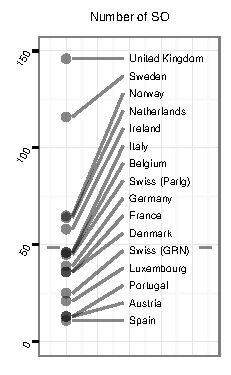
\includegraphics{in_progress_files/figure-latex/unnamed-chunk-2-1.pdf}
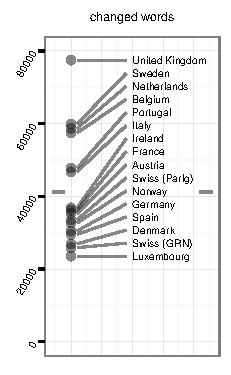
\includegraphics{in_progress_files/figure-latex/unnamed-chunk-2-2.pdf}
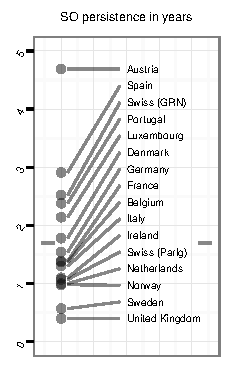
\includegraphics{in_progress_files/figure-latex/unnamed-chunk-2-3.pdf}
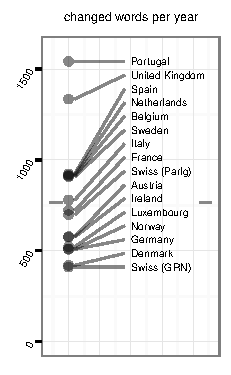
\includegraphics{in_progress_files/figure-latex/unnamed-chunk-2-4.pdf}

The graphics above give a brief overview of four basic variables in the
data set. They show they show the value as well as the rank for the
number of SO in the data set, the amount of changed that occured to
those SO, how many years it takes on average until it is replaced by a
new version, the average amount of words that are changed per year.

First of all, all countries under consideration do change their SO
frequently and to an substantial amount. On average SO are changed every
1.7 years with an change rate of approximatly 770 words per year. Within
the variables there is considerable variance as well. UK and Sweden are
the most frequent changers with more than one version per year while
Austria's SO have an exceptional high lifespan with over 4.5 years - in
the UK all matters seem to require a change of SO even the creation or
disolving of a single committee while in Austria changing the SO
requires a super majority. In regard to the amount changed especially
Portugal and UK seem to play a special role. In addition to beeing a
hyper-frequent changer UK also manages to change much more than other
countries. One reason for this is that in UK all rules for the Grand
Committees for Northern Ireland. Scotland and Wales are speleld out
explicitly and redundantly. Portugal on the other hand had very view
changes (13) since 1976 with one reform beeing extremely extensive so
that over time the Portugese change rate might wander nearer towards the
other countries.

\pagebreak{}

\section{Reforms per country}\label{reforms-per-country}

In the following the the length, topical distribution as well as the
amount of change and the type of change are plotted country by country.

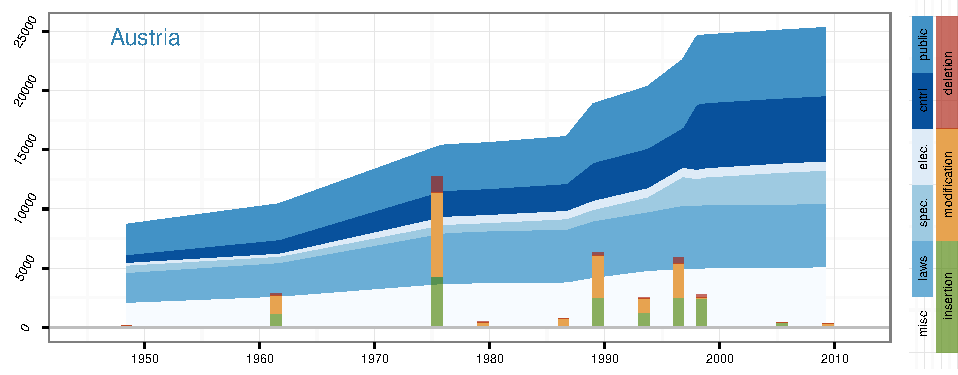
\includegraphics{in_progress_files/figure-latex/unnamed-chunk-5-1.pdf}
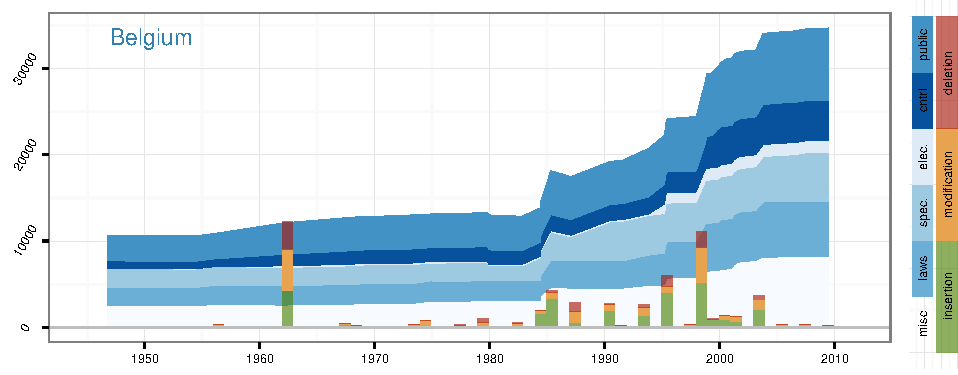
\includegraphics{in_progress_files/figure-latex/unnamed-chunk-5-2.pdf}
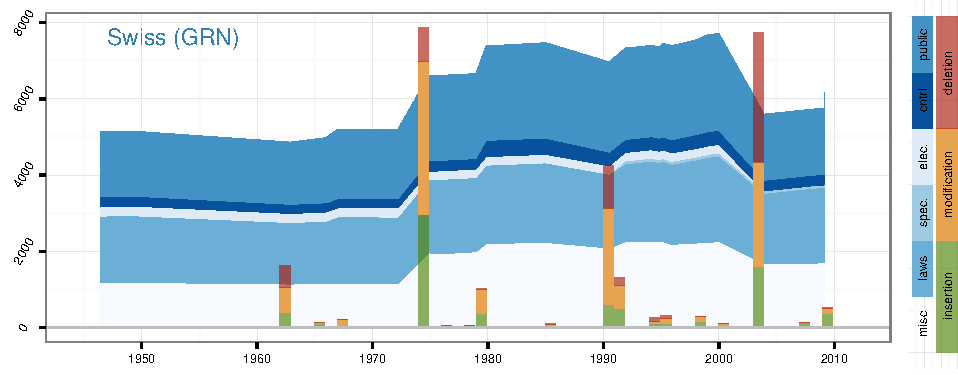
\includegraphics{in_progress_files/figure-latex/unnamed-chunk-5-3.pdf}
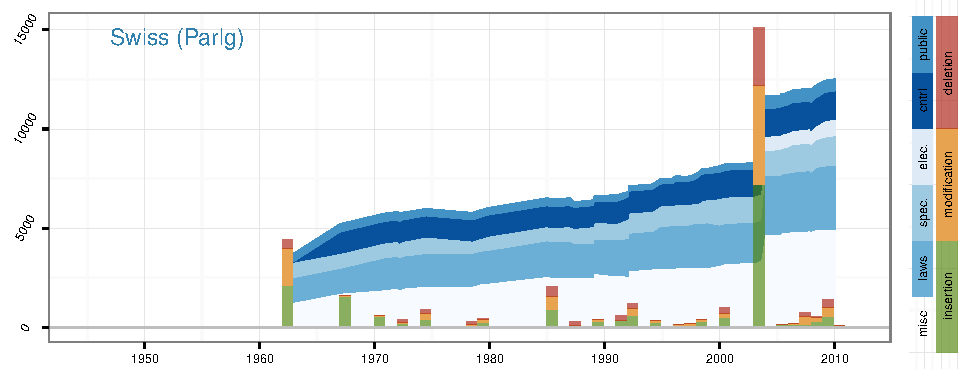
\includegraphics{in_progress_files/figure-latex/unnamed-chunk-5-4.pdf}
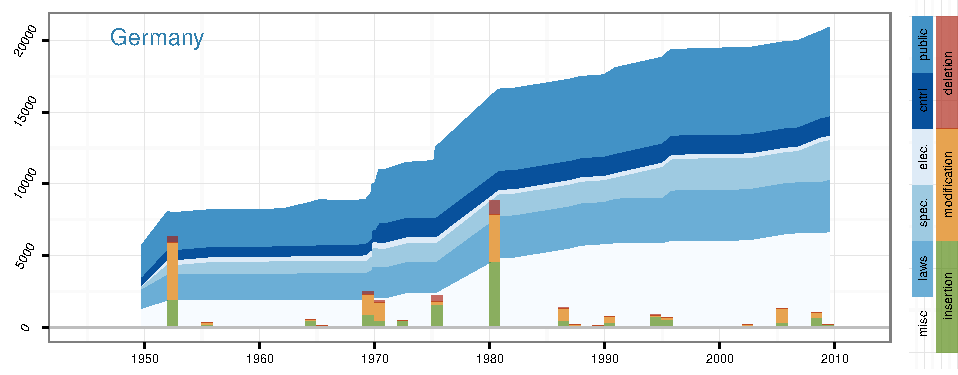
\includegraphics{in_progress_files/figure-latex/unnamed-chunk-5-5.pdf}
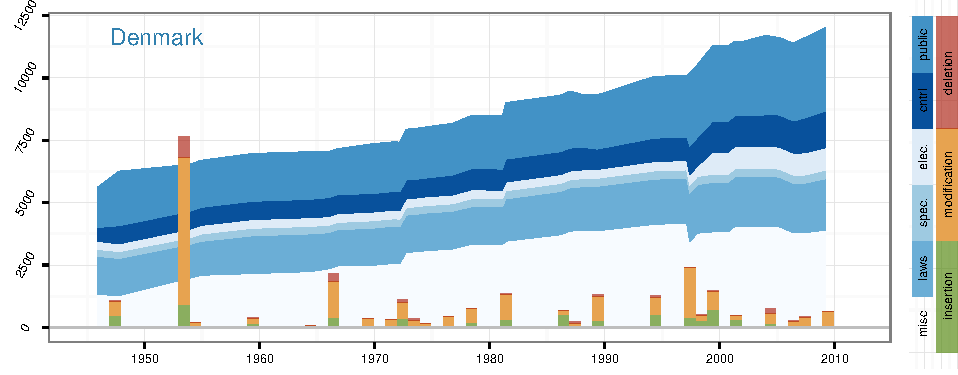
\includegraphics{in_progress_files/figure-latex/unnamed-chunk-5-6.pdf}
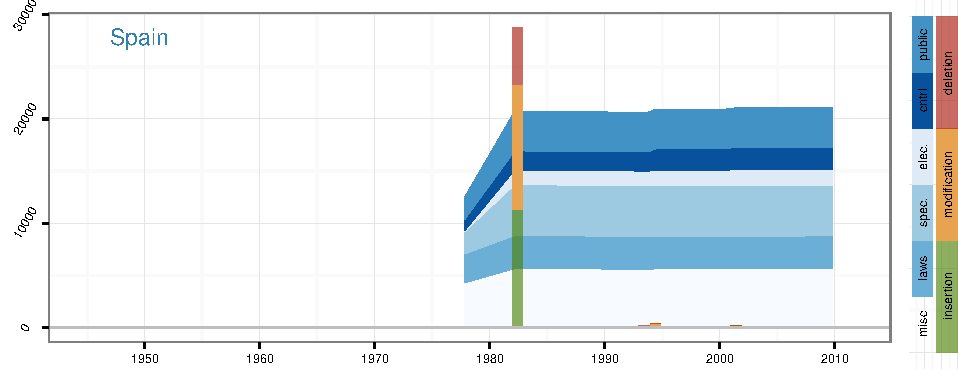
\includegraphics{in_progress_files/figure-latex/unnamed-chunk-5-7.pdf}
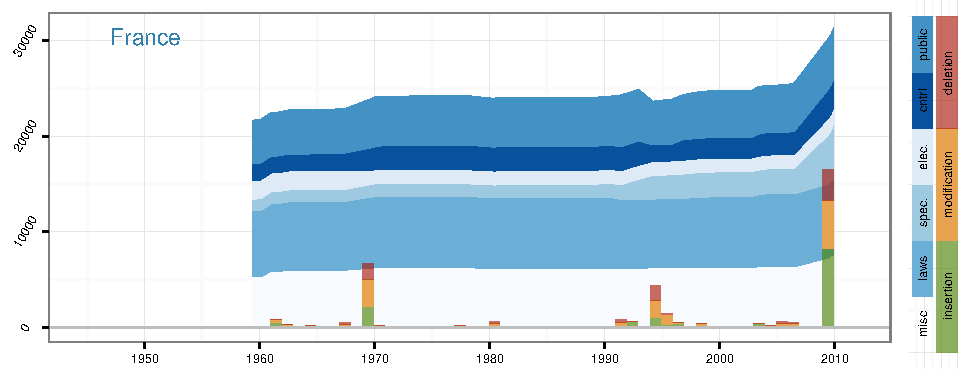
\includegraphics{in_progress_files/figure-latex/unnamed-chunk-5-8.pdf}
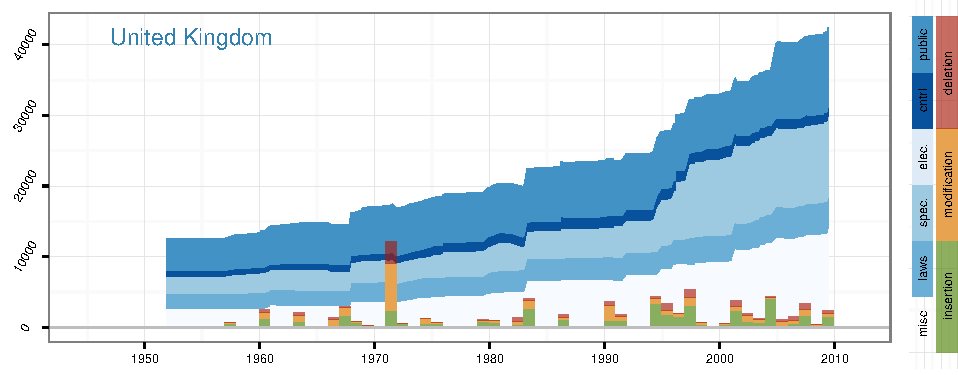
\includegraphics{in_progress_files/figure-latex/unnamed-chunk-5-9.pdf}
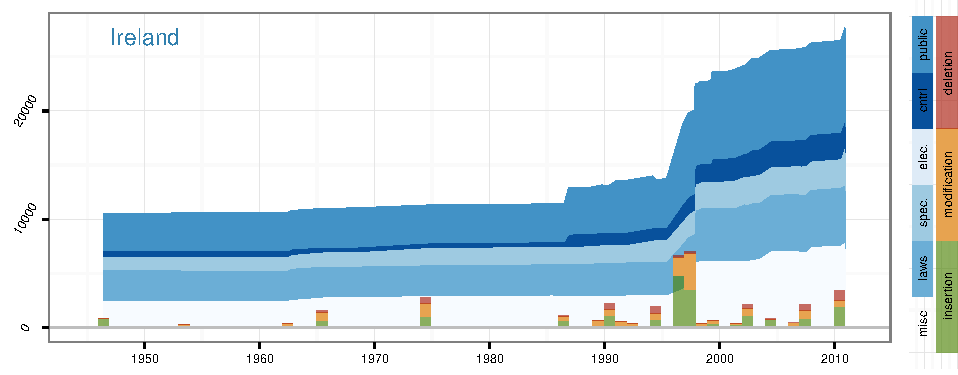
\includegraphics{in_progress_files/figure-latex/unnamed-chunk-5-10.pdf}
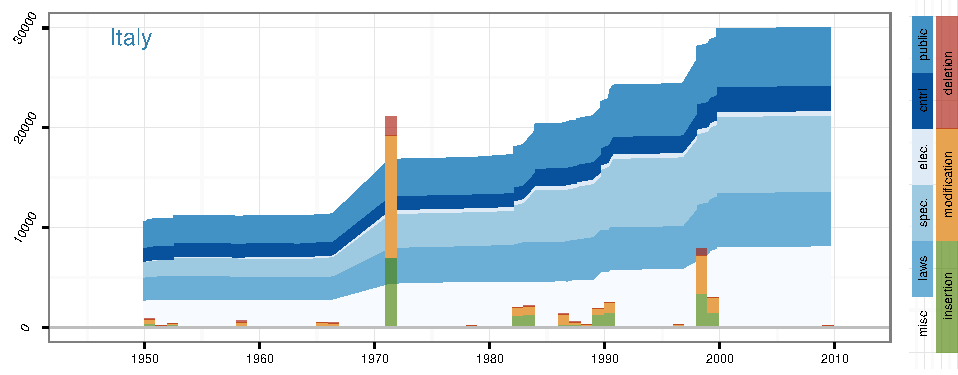
\includegraphics{in_progress_files/figure-latex/unnamed-chunk-5-11.pdf}
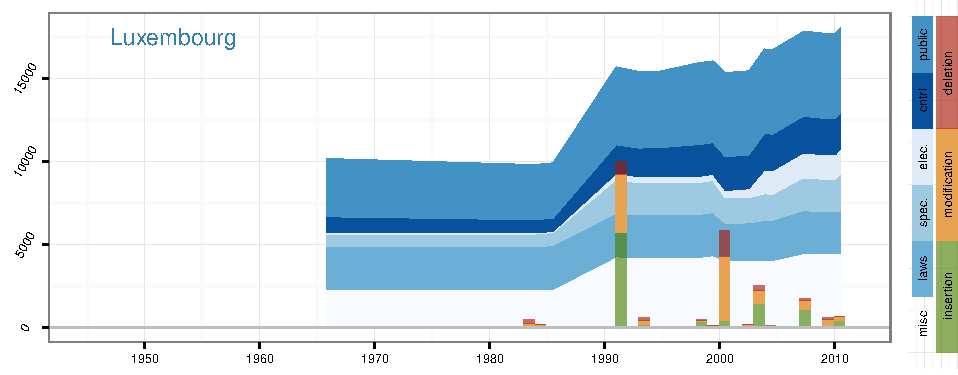
\includegraphics{in_progress_files/figure-latex/unnamed-chunk-5-12.pdf}
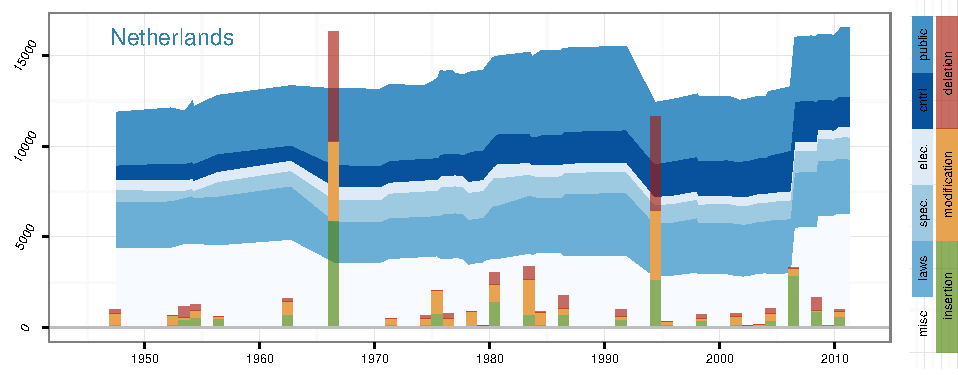
\includegraphics{in_progress_files/figure-latex/unnamed-chunk-5-13.pdf}
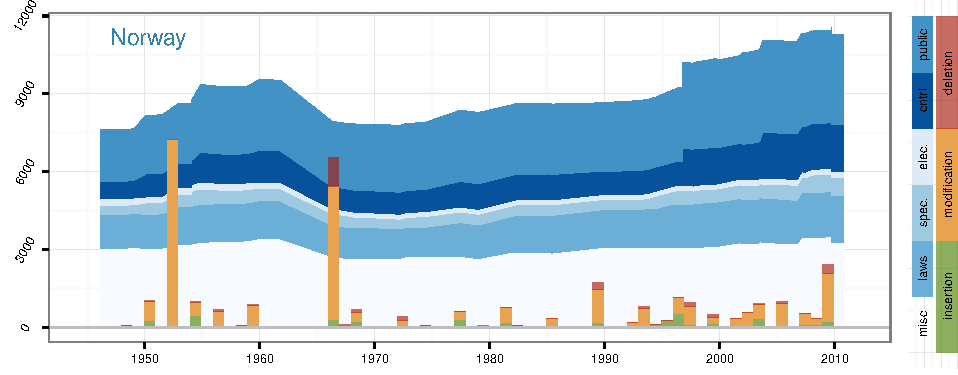
\includegraphics{in_progress_files/figure-latex/unnamed-chunk-5-14.pdf}
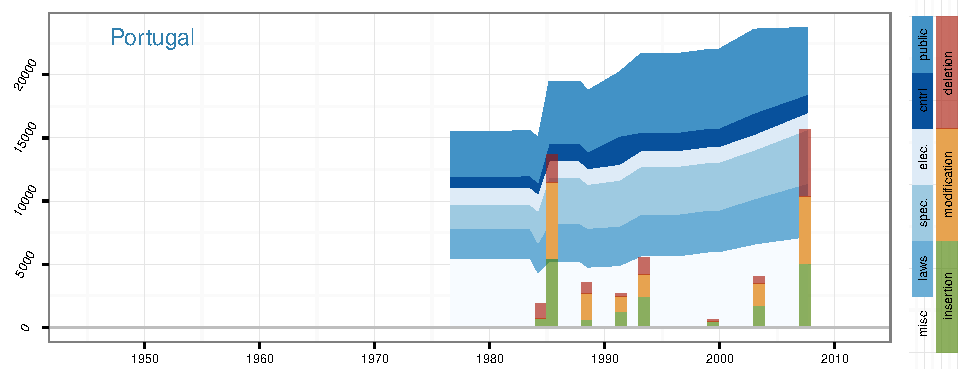
\includegraphics{in_progress_files/figure-latex/unnamed-chunk-5-15.pdf}
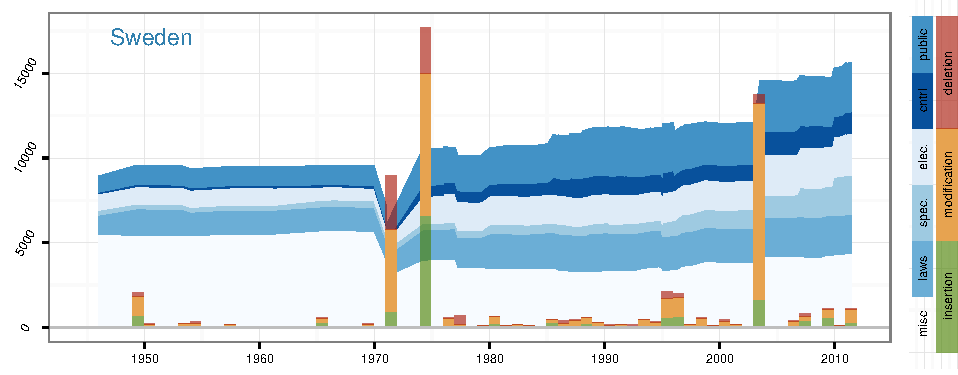
\includegraphics{in_progress_files/figure-latex/unnamed-chunk-5-16.pdf}

\pagebreak{}

\section{dutiestodo}\label{dutiestodo}

\begin{verbatim}
## ==========================================================================
\end{verbatim}

\begin{verbatim}
## file copied to: 
## Z:/Geschäftsordnungen/Papiere und Konferenzen/2015_corpus_coding/in_progress/
\end{verbatim}

\begin{verbatim}
## [1] TRUE
\end{verbatim}

\end{document}
